%-- Add sections and your outline will be created automatically --%
\subsection{Water collapse}

% Frame starts a new slide
\begin{frame}
    \frametitle{Water collapse}
\begin{itemize}
\item Barrier removed instantaneously at $t = 0$; flow driven by gravity
\item Inviscid, multi-material flow, mesh adaptivity
\item Static detectors to compare with benchmark lab data
\item Run time: 2 hr.
\end{itemize}

\begin{figure}
\centering
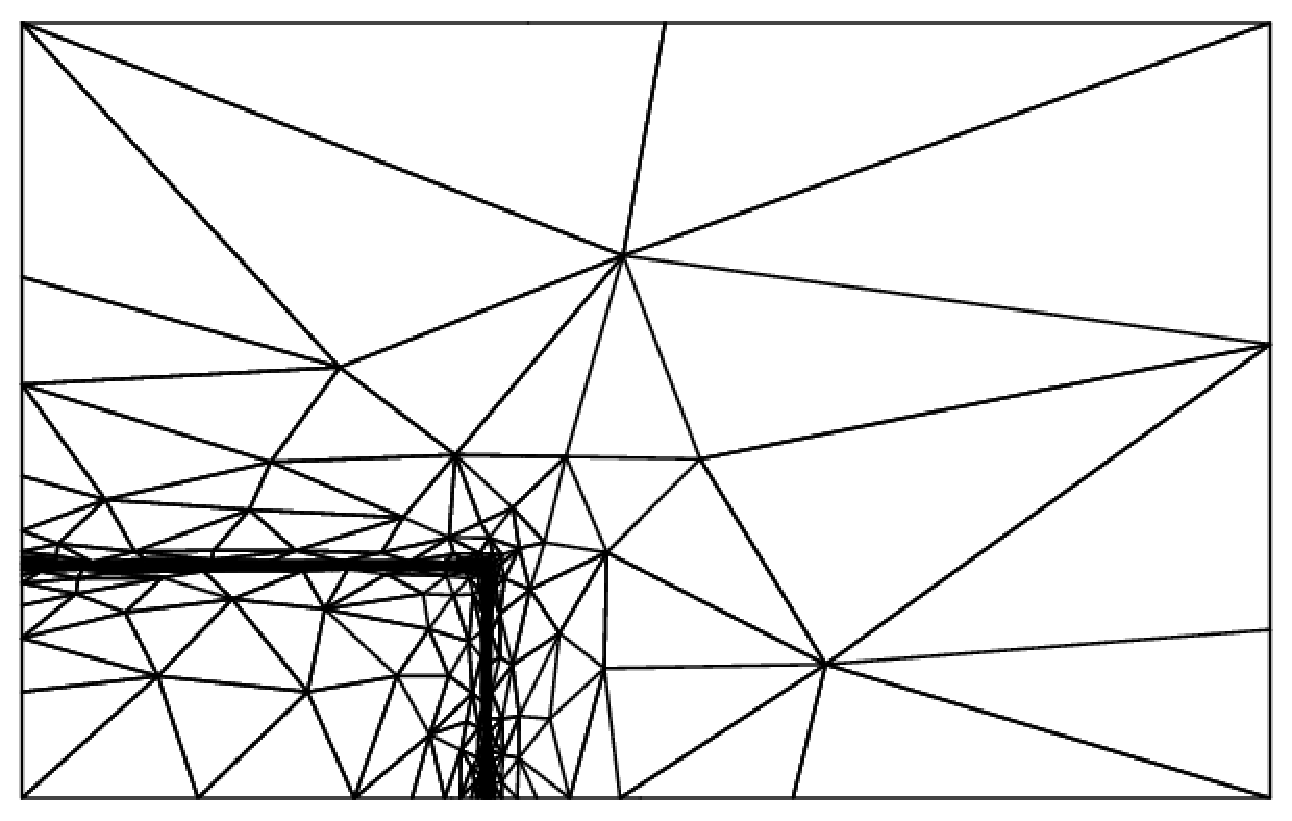
\includegraphics[width=0.5\textwidth, clip=true]{./water_collapse/water_collapse_0_mesh.pdf}
\caption{Initial unstructured adapted mesh for water collapse problem.}
\end{figure}

\end{frame}
%
\begin{frame}
    \frametitle{Water collapse}

\begin{figure}
\centering
\subfigure[$t=0.5$]{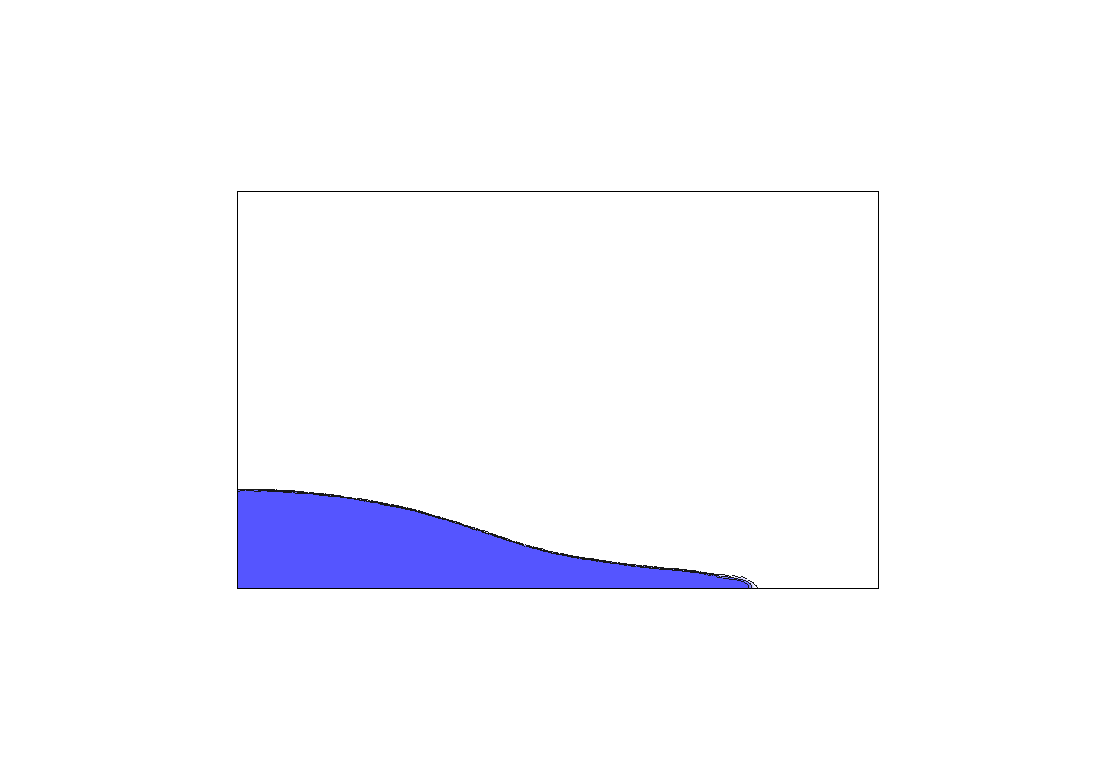
\includegraphics[width=0.275\textwidth, trim=7.5cm 6.5cm 7.5cm 6.5cm, clip=true]{./water_collapse/water_collapse_100.png}}
\subfigure[$t=1.0$]{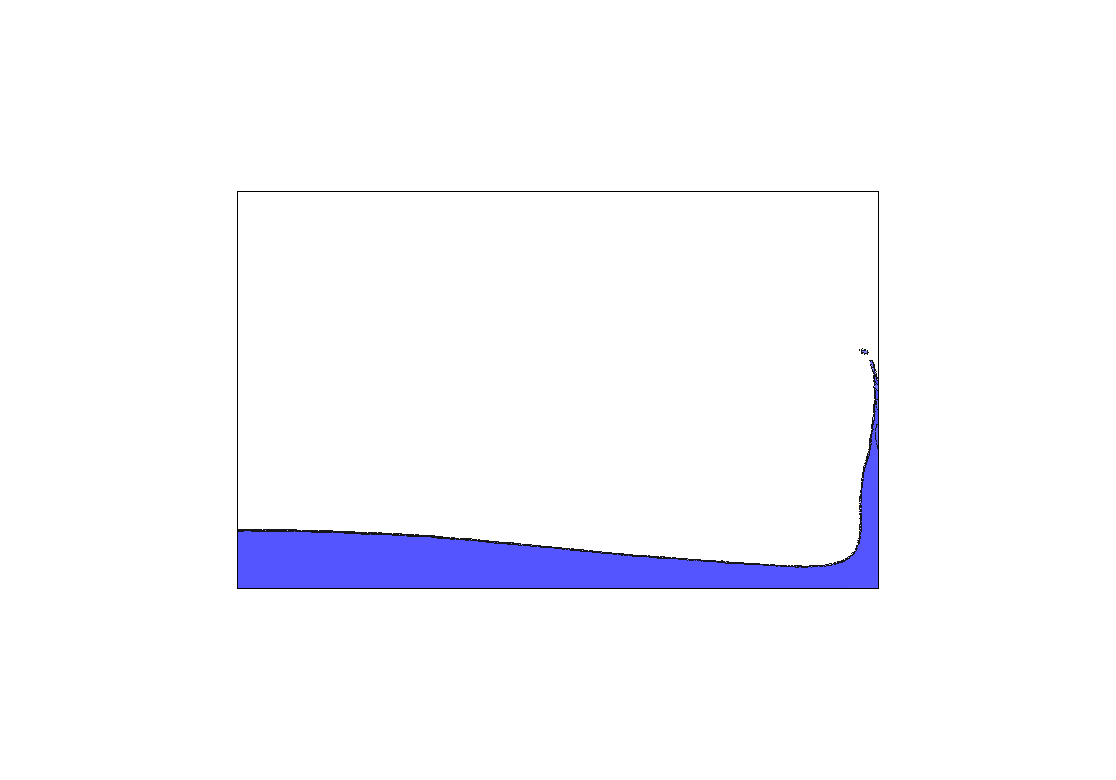
\includegraphics[width=0.275\textwidth, trim=7.5cm 6.5cm 7.5cm 6.5cm, clip=true]{./water_collapse/water_collapse_200.png}}
\subfigure[$t=1.5$]{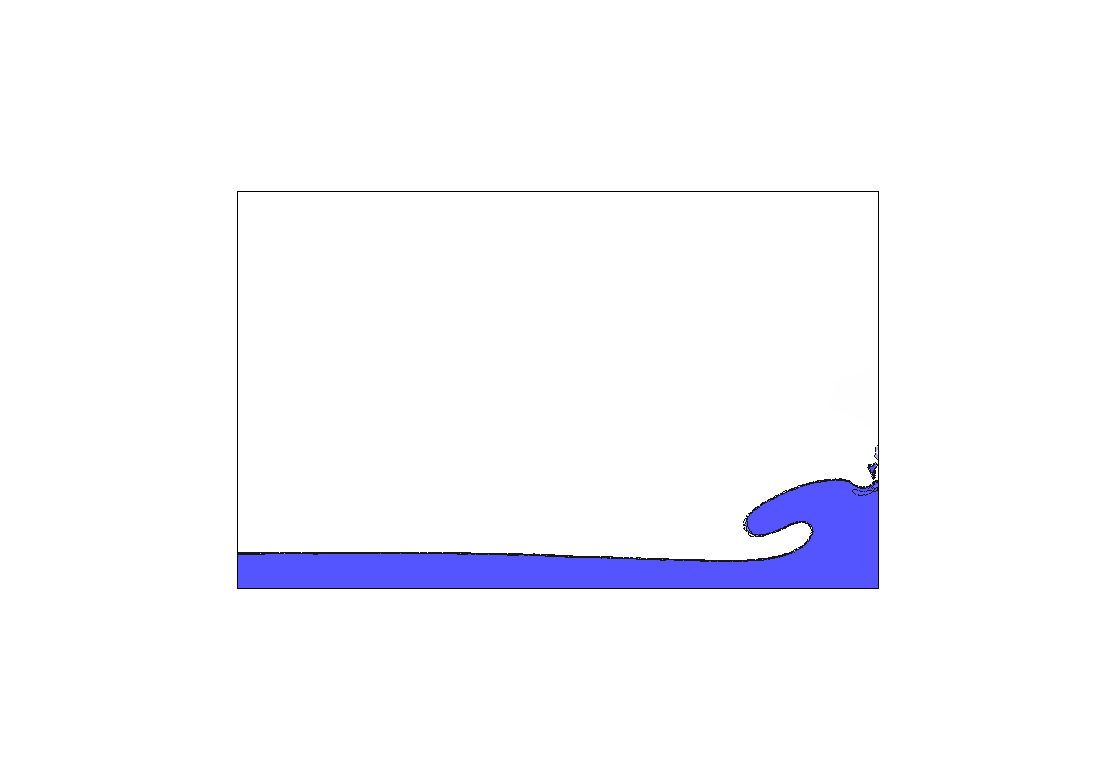
\includegraphics[width=0.275\textwidth, trim=7.5cm 6.5cm 7.5cm 6.5cm, clip=true]{./water_collapse/water_collapse_300.png}}
\subfigure[$t=1.75$]{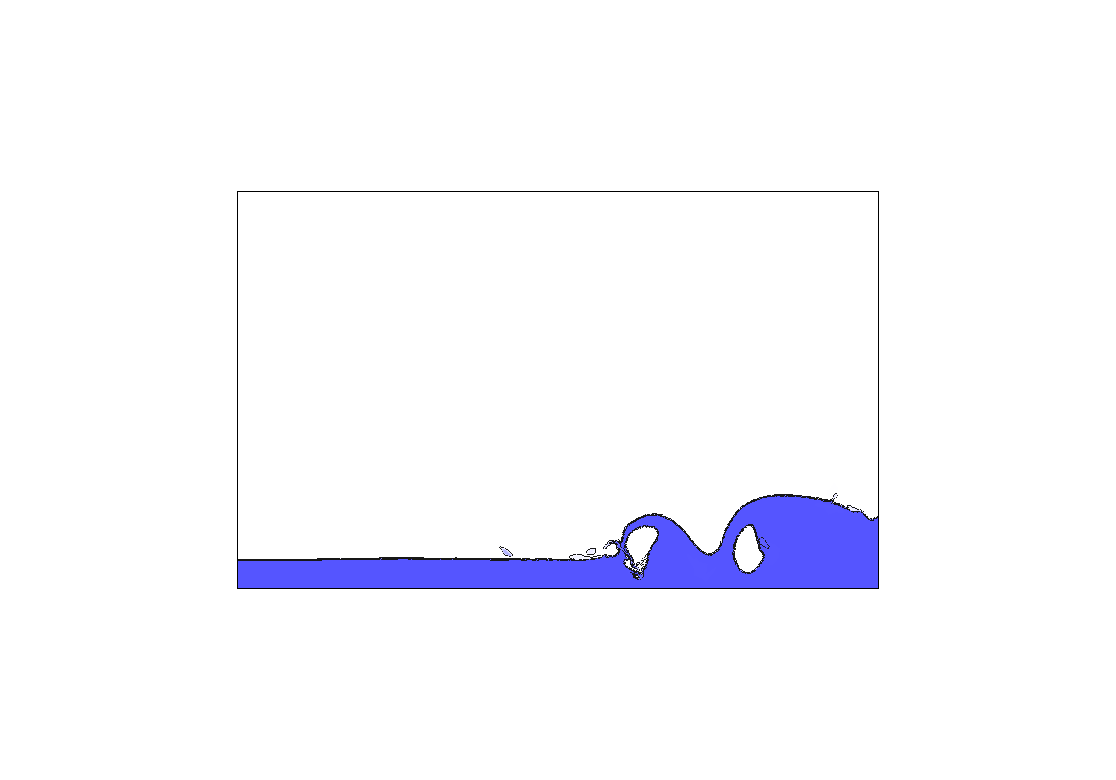
\includegraphics[width=0.275\textwidth, trim=7.5cm 6.5cm 7.5cm 6.5cm, clip=true]{./water_collapse/water_collapse_350.png}}
\subfigure[$t=2.25$]{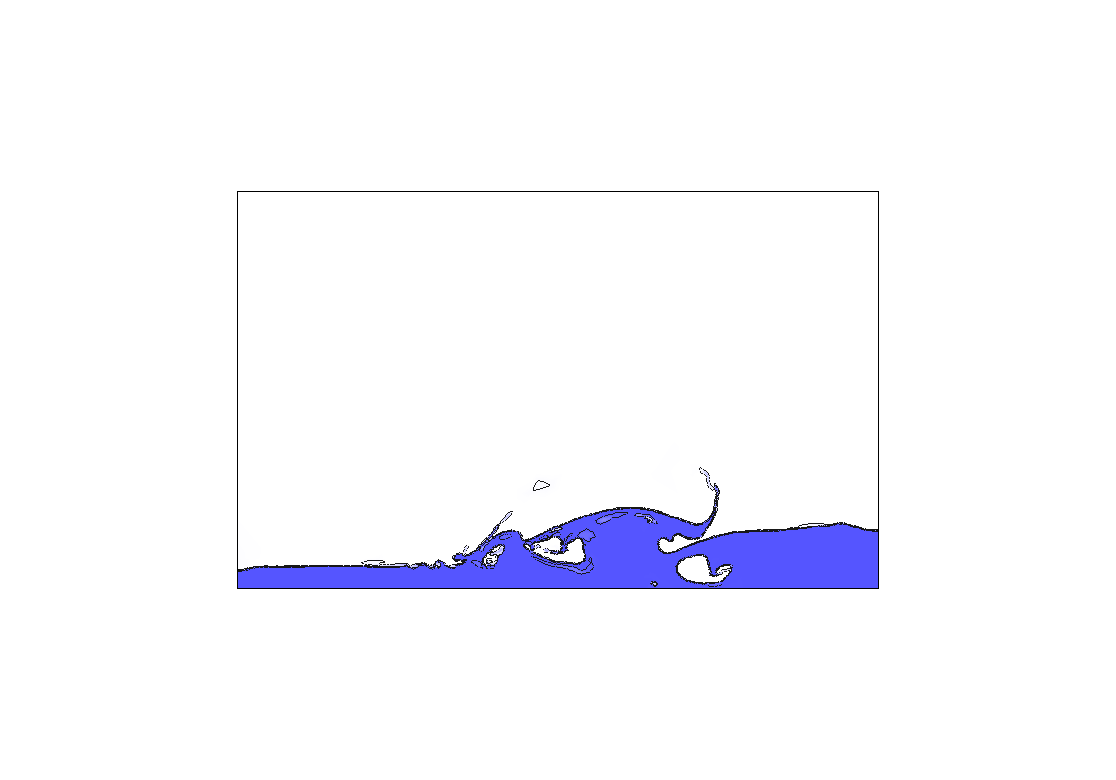
\includegraphics[width=0.275\textwidth, trim=7.5cm 6.5cm 7.5cm 6.5cm, clip=true]{./water_collapse/water_collapse_450.png}}
\subfigure[$t=2.5$]{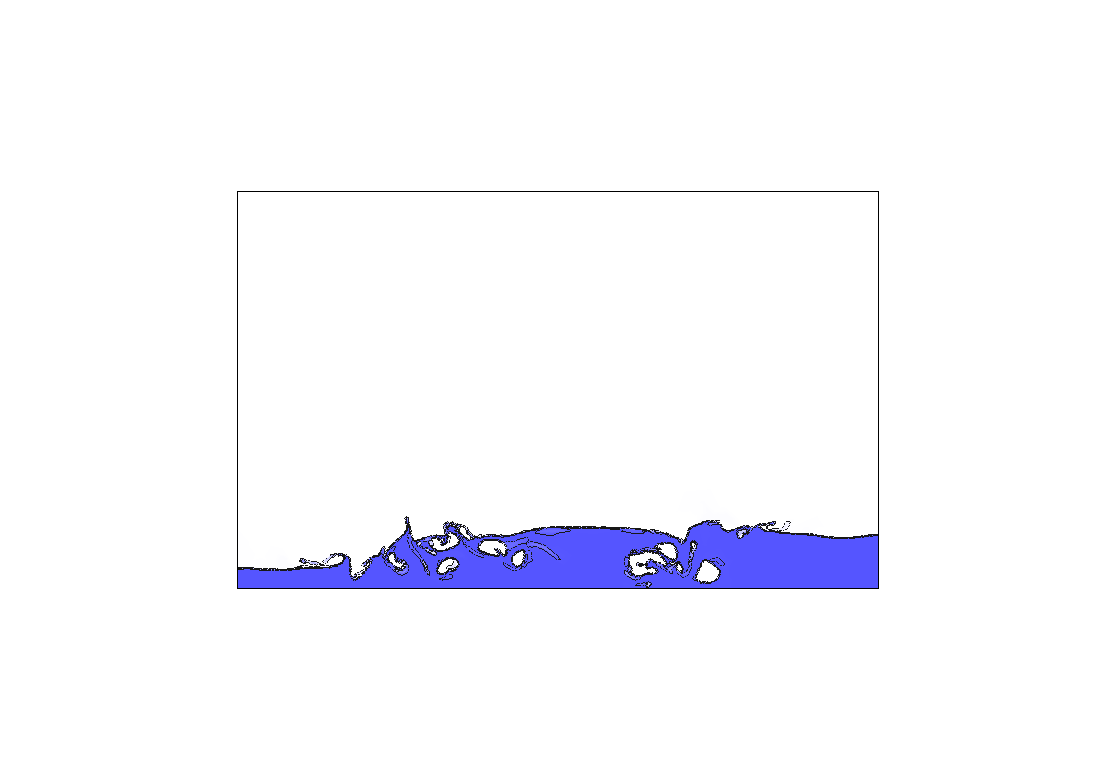
\includegraphics[width=0.275\textwidth, trim=7.5cm 6.5cm 7.5cm 6.5cm, clip=true]{./water_collapse/water_collapse_500.png}}
\caption{The evolution of the water volume fraction over several timesteps.  The presence of water is indicated as a blue region and the interface to the air is delineated by the contours (in black).}
\end{figure}

\end{frame}
%
\begin{frame}
    \frametitle{Water collapse}
\begin{itemize}
\item Post-processing scripts output several plots, e.g. comparison of water depth to experimental data
\end{itemize}
\begin{figure}
\centering
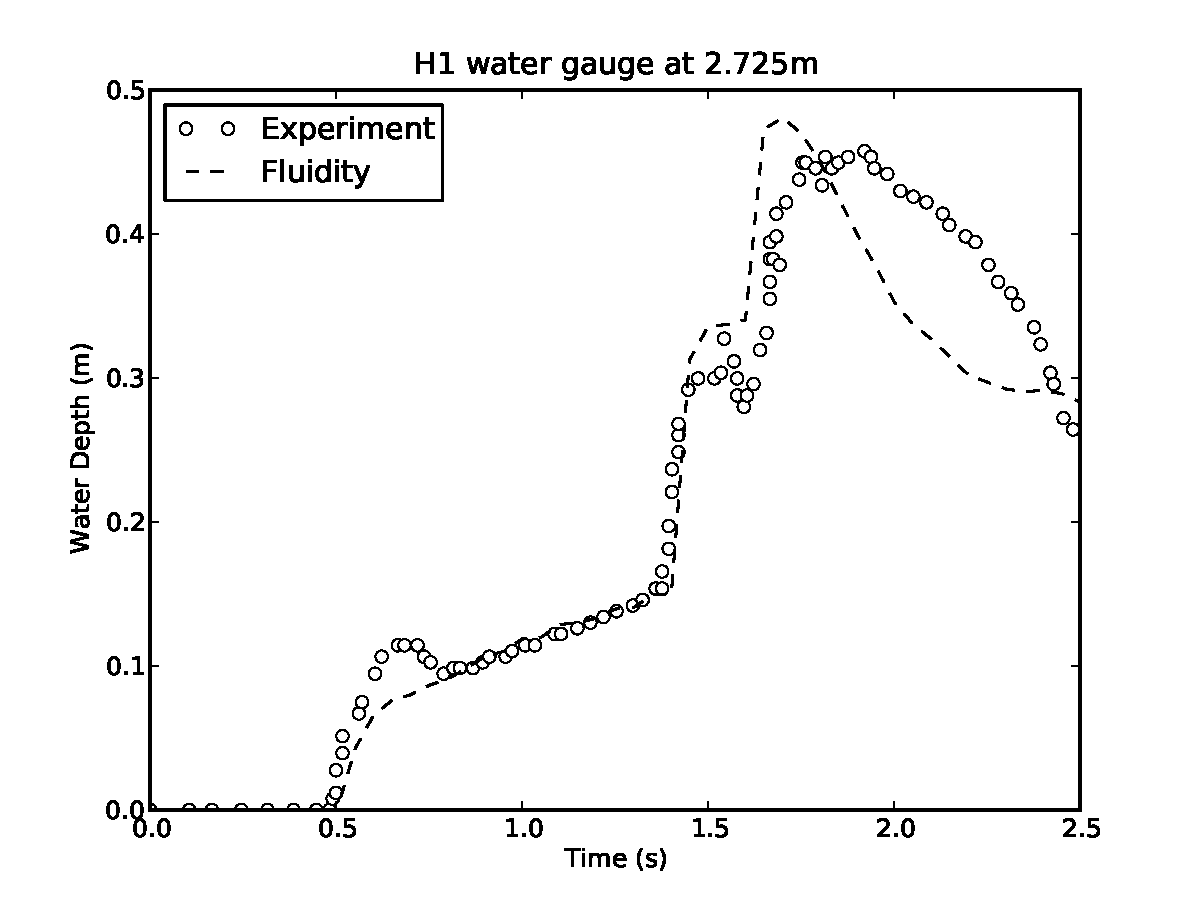
\includegraphics[width=0.5\textwidth]{./water_collapse/water_gauge_H1.pdf}
\caption{Comparison with experimental depth gauge data at $x = 2.725 \, $m.}
\end{figure}

\end{frame}
%
\begin{frame}
    \frametitle{Water collapse, exercises}
\begin{itemize}
\item Disable the adaptivity option to run on a fixed mesh.
\item Alter the water/air viscosity/density.
\item Modify the tank geometry.
\end{itemize}

\end{frame}
